\documentclass[../root]{subfiles}
\graphicspath{{_images/}{../_images/}}

\begin{document}

    \chapter{Can Small Incentives Have Large Effects? The Impact of Taxes versus Bonuses on Disposable Bag Use}

    \begin{shortsummary}
        \begin{itemize}
            \item \authoryear{Homonoff2018}
            \item \RQ{Does loss-aversion work also in the field for very small stakes incentives?}
            \item \answer{DID/cross-sectional evaluations of two real- world policies aimed at reducing disposable bags use in the U.S.}
            \item \result{Consistent with a model of loss aversion: tax for disposable bags decreased usage by over 40 percentage points, while bonus for reusable bags generated little effect.}
        \end{itemize}
    \end{shortsummary}

    \section{Introduction}

    \paragraph{Motivation: How to make small incentives to have large effects on behavior?}

    \begin{itemize}
      \item Americans consume 100 billion plastic bags each year: 1.5 trillion (Clapp and Swnason 2009).
      \begin{itemize}
        \item Only 5.2\% of plastic bags in the U.S. in 2005 were actually recycled (Environmental Protection Agency).
        \item Policymakers hav passed a variety of policies to curb disposable bag consumption.
      \end{itemize}
      \item Loss-aversion
      \begin{itemize}
        \item Individuals perceive losses more strongly than gains (Kahneman and Tversky 1979).
        \item Research that aims to document this asymmetry is growing.
        \begin{itemize}
          \item Field (2009)
          \item Fryer et al. (2012)
          \item Hossain and List (2012)
        \end{itemize}
        \item How about \textbf{small incentives}?
        \begin{itemize}
          \item Less is known about whether this asymmetry holds in the field for very small stakes incentives.
          \begin{itemize}
            \item Too small incentives may demotivating by crowding out an individual's intrinsic motivation (Gneezy and Rustichini 2000a, b; Gneezy, Meier, and Rey-Biel 2011).
          \end{itemize}
        \end{itemize}
      \end{itemize}
      \item Contribution
      \begin{itemize}
        \item This paper considers loss-framed nudges in a new policy where very small incentives set.
      \end{itemize}
    \end{itemize}

    \paragraph{Data and Identification}

    \begin{itemize}
      \item Comparision between two real-world policies aimed at reducing the use of disposable shopping bags.
      \begin{itemize}
        \item Tax on disposable bag use: Washington, DC and Maryland.
        \item Bonus for for reusable bag use: several stores in the area voluntarily offered a bonus for reusable bag use.
      \end{itemize}
      \item A unique large dataset on individual-level use of disposable and reusable bags.
      \begin{itemize}
        \item shopping behavior of grocery store customers during the months before and after the implementation of disposable-bag tax in three counties in the Washington Metropolitan Area.
      \end{itemize}
      \item Identification: DID and cros-sectional regression analysis.
    \end{itemize}

    \paragraph{Sum of the results}

    \begin{itemize}
      \item Loss-framing: fees
      \begin{itemize}
        \item The fraction of customers that used at least one disposable bag per shopping trip in Montgomery County: 82\% to 40\% after the tax.
        \item Customers who continued to use them after the tax used fewer bags per trip.
        \item Even though it was a small size of the financial incentive, the effects are critical.
      \end{itemize}
      \item Gain-framing: bonus
      \begin{itemize}
        \item Almost no impact on disposable bag use: 82 verse 84\%.
      \end{itemize}
      Taken together, the results are consistent with a model of loss aversion.
      \item Alternative explanations:
      \begin{itemize}
        \item Awareness of the bonus and the tax.
        \item Changes in consumer attitudes toward disposable bag use.
      \end{itemize}
    \end{itemize}

    \section{Background}

    \paragraph{Disposable Bag Regulations}

    \begin{itemize}
      \item In an effort to reduce pollution, policymakers considered policies to reduce disposable bag consumption.
      \item Policies that requre retailers to charge customers for their plastic bag consumption.
      \begin{itemize}
        \item This policy started in the early 2000s in several countries in Europe, Asia, and Africa.
        \item Washington, DC is the first city in the U.S. to charge a fee (Anacostia River Cleanup and Protection Act).
        \item As of January 1, 2010, all food retailers in the district are requred to charge \$.05 per single-use plastic or paper bag.
        \item 2 years later, Montgomery County, Maryland enacted the similar regulation.
      \end{itemize}
      \item Voluntary introduction of a bonus for reusable bag.
      \begin{itemize}
        \item Prior to the implementation, half of the grocery stores in the Washington Metropolitan Area with the largest market share offered customers a \$.05 bonus for each reusable bag.
      \end{itemize}
    \end{itemize}


    \section{Models}

    \paragraph{Basic Setting}

    \begin{itemize}
      \item The utility of the consumer $i$ is defined as follows:
      \begin{figure}[ht]
        \centering
        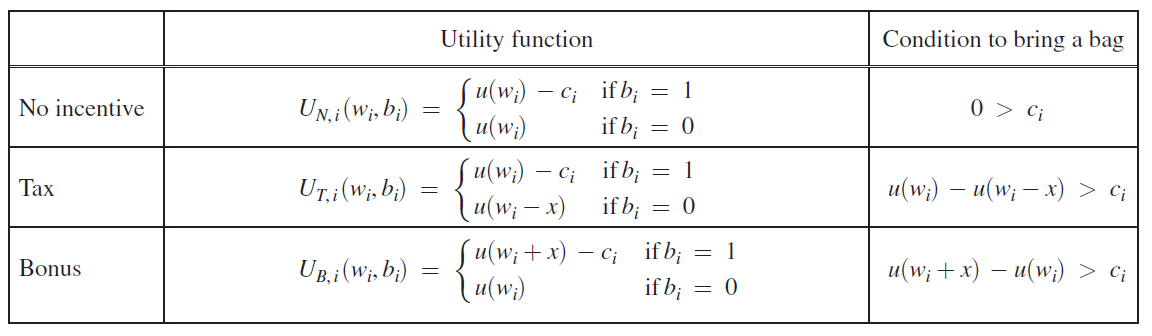
\includegraphics[scale = .8]{0807tanji/model}
      \end{figure}
      where
      \begin{itemize}
        \item $w_i$: consumer's wealth.
        \item $b_i$: indicator for cosumer bringing a reusable bag.
        \item $c_i$: cost for bringing a reusable bag.
      \end{itemize}
      \item Utility is additively separable between $c$ and $w$.
      \item This paper consider the effect of tax and bonus with a very small amount $x$.
    \end{itemize}

    \subsection{Neoclassical Model}

    \begin{itemize}
      \item Standard economic theory predicts that if $c_i$ is also very small, a small $x$ could still have a large effect on behavior.
      \item Assume that utility is strictly increasing and weakly concave, or $u'(w) > 0$ and $u"(w) \leq 0$, then we can explain the behavior such that individuals react to loss-framing.
      \begin{itemize}
        \item Rabin (2000): Individuals must be approximately risk-neutral over small stakes: incentives of \$.05 per bag may be negligible.
      \end{itemize}
      Thus, we assume that utility is linear: $u(w_i) = \gamma w_i$.
      $\Rightarrow$ the tax plicy and the bonus policy derive exactly the same behavior.
    \end{itemize}

    \begin{figure}[ht]
      \centering
      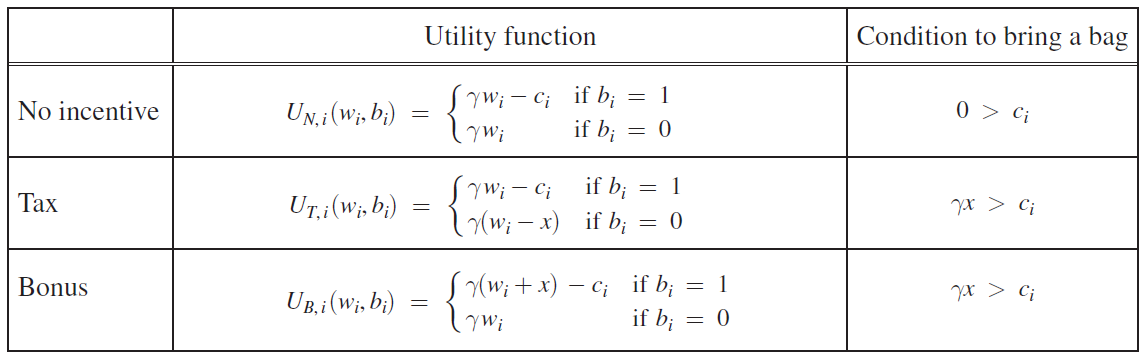
\includegraphics[scale = .8]{0807tanji/modelA}
    \end{figure}

    \subsection{Reference-Dependent Model}

    \begin{itemize}
      \item A simple reference-dependent utility function.
      \[
      u(w_i) = \begin{cases}
        \gamma (w_i - w^*) & \text{ if } w_i > w^* \\
        \alpha \gamma (w_i - w^*) & \text{ if } w_i \leq w^*
    \end{cases},
    \text{ where }\alpha > 1.
      \]
    \end{itemize}

    \begin{figure}[ht]
      \centering
      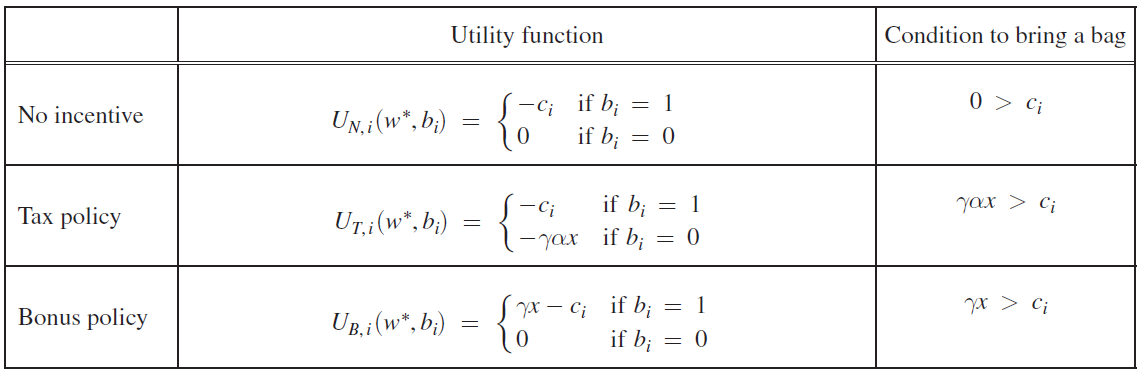
\includegraphics[scale = .8]{0807tanji/modelB}
    \end{figure}


    \section{Data}

    \paragraph{A unique dataset of bag use in the Washington Metropolitan Area}

    \begin{itemize}
      \item An exit survey of a grocery store: individual-level data on the number and type of bags each customer used.
      \begin{itemize}
        \item Visually assessable demographic characteristics: sex, race, \ldots.
        \item Researchers visited each store in 30 minute shifts, randomizing the time and location on weekdays.
        \item Final sample: on average 9 visits $\times$ 16,251 individual customers.
      \end{itemize}
      \item Sample period and cross-sectional choice
      \begin{itemize}
        \item The disposable bag tax in Montgomery was implemented on January 1, 2012: the sample includes three months before and after then.
        \item 16 stores spanning 3 different counties, with a different tax policy regime: MoWashington, DC, Arlington County, Virginia, and Montgomery.
        \item The stores belong to 4 of the largest chains in the Washington Metropolitan Area: 2 of which offer \$.05 bonuses for reusable bags both before and after the implementation.
        \item Notations
        \begin{enumerate}
          \item All four chains had locations in all the counties.
          \item Stores in the sample has similar demographic characteristics.
          \item All sample stores had a parking lot and were accessible by metro.
          \item The stores were the same size.
          \item All stores sold reusable bags.
          \item There are some organic stores are included in the sample.
        \end{enumerate}
      \end{itemize}
    \end{itemize}

    \begin{figure}[ht]
      \centering
      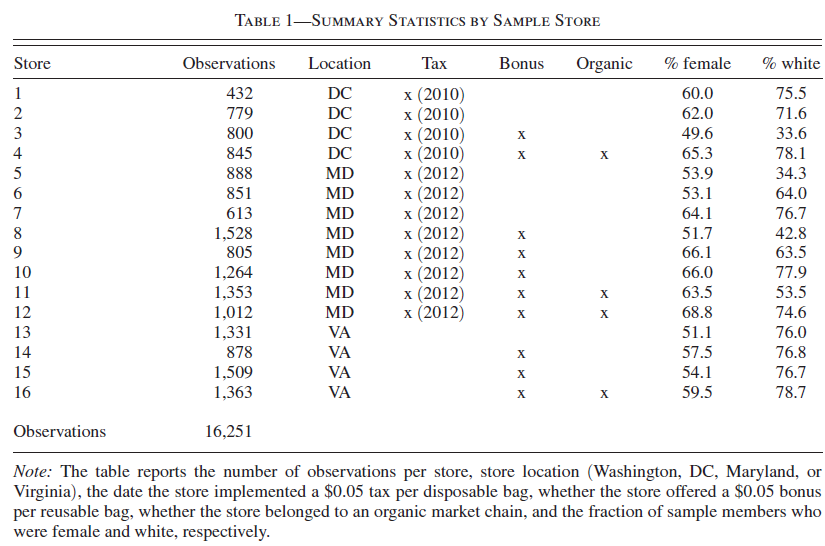
\includegraphics[scale = 1]{0807tanji/T1}
    \end{figure}

    \paragraph{Supplimental Survey datasets}

    To investigate various mechanisms, they obtained following datasets:

    \begin{itemize}
      \item In-person surveys of customers
      \begin{itemize}
        \item exit-survey during September and Octover of 2011 and March of 2012, 1,496 respondants.
        \item Information about the number of disposable/reusable bags, awareness of the bonus/tax, the degree of encouragement to use reusable ones, \ldots.
      \end{itemize}
      \item Online survey to test customers' response to hypothetical disposable bag regulations: MTurk.
      \item Transaction-level data.
    \end{itemize}


    \section{The Relative Effectiveness of the Tax and Bonus Policies}

    \subsection{Tax Policy}

    \paragraph{Comparison of the average usage}

    \begin{itemize}
      \item Bag use in Montgomery changed dramatically after the implement: increase in usage of reusable bags and decrease in that of disposable ones.
      \begin{itemize}
        \item the percent of customers using each type of bag or no bags (extensive margin)
        \item the number of bags each customer | he/she uses the bag (intensive margin)
        \item the unconditional number of bags per customer (overall demand)
      \end{itemize}
    \end{itemize}

    \begin{figure}[ht]
      \centering
      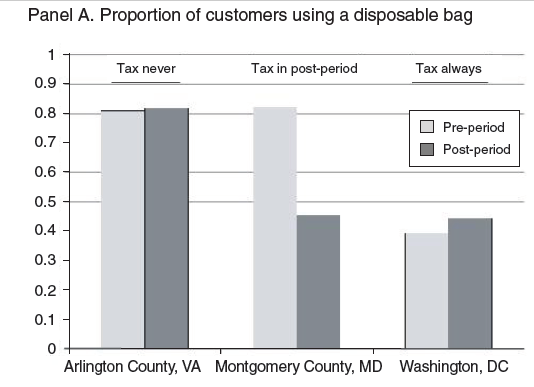
\includegraphics[scale = .8]{0807tanji/F3A}
      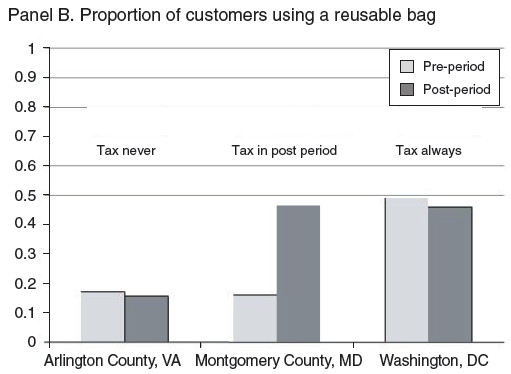
\includegraphics[scale = .8]{0807tanji/F3B}
    \end{figure}

    \paragraph{DID analysis}

    \begin{itemize}
      \item DID strategy strategy controlling for various individual characteristics and location-level controls:
      \[
      Y_{isdt} = \alpha + \beta \text{MD} \times \text{Post}_{st} + \gamma \text{Post}_{t} + \eta Z_s + \lambda X_i + \delta Q_d + \epsilon_{isdt}
      \]
      for individual $i$ shopping in location $s$ during time of day $d$ at time period $t$.
      \item (Table 3): The tax caused a decrease in the proportion of customers using at least one disposable bag by 41.7 percentage points.
      \begin{figure}[ht]
        \centering
        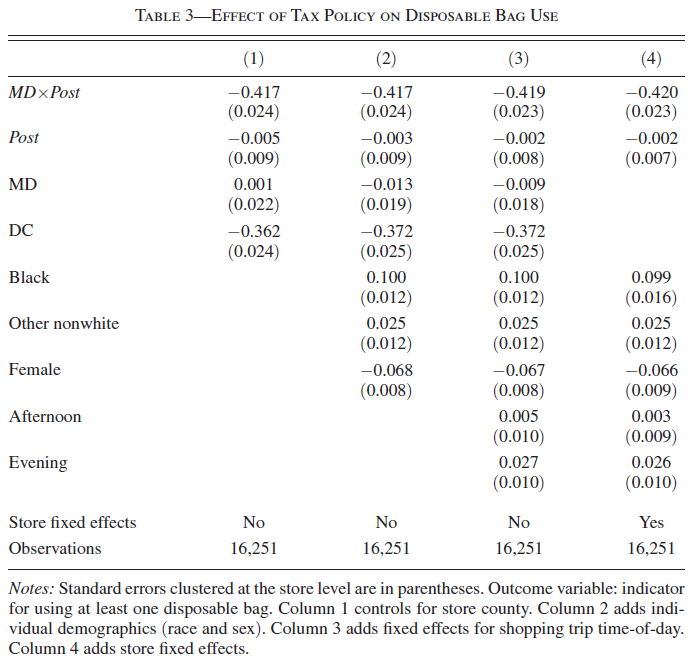
\includegraphics[scale = .8]{0807tanji/T3}
      \end{figure}
      \item (Table 4) Extensive margin: Tax
      \begin{itemize}
        \item decreased usage of disposable bag by 42.0 percentage points
        \item increased that of reusable ones by 32.7 percentage points
        \item increased that of no bags by 11.1 percentage points
      \end{itemize}
      \item Intensive margin: Tax
      \begin{itemize}
        \item decreased the number of bags used by disposable bag users decreased by .22.
        \item increased reusable: by .15 bags.
      \end{itemize}
      \begin{figure}[ht]
        \centering
        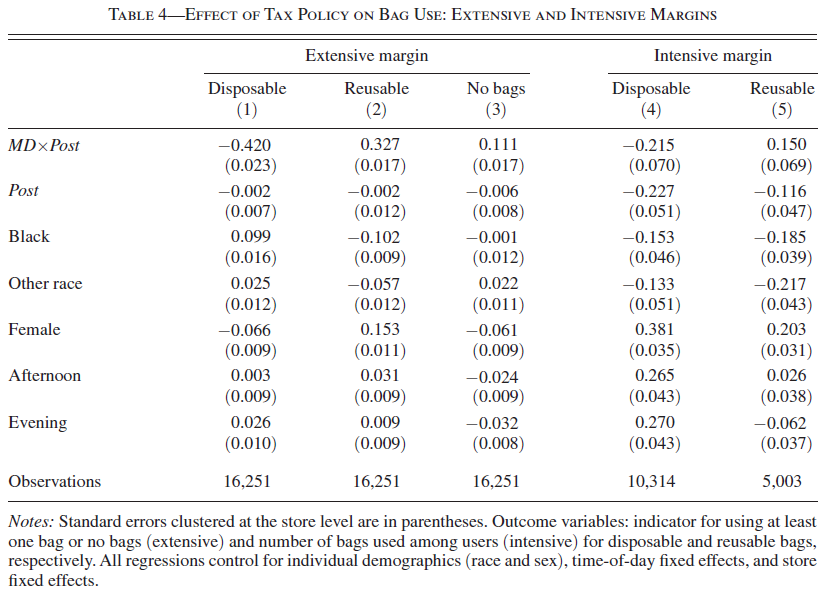
\includegraphics[scale = .8]{0807tanji/T4}
      \end{figure}
      \item (Table 5) Overall effect on demand.
      \begin{itemize}
        \item Linear demand model
        \item Double-hardle model: $E[y | x] = E[y | x, y > 0] \times \text{Pr}(y > 0 | x)$.
        \begin{figure}[ht]
          \centering
          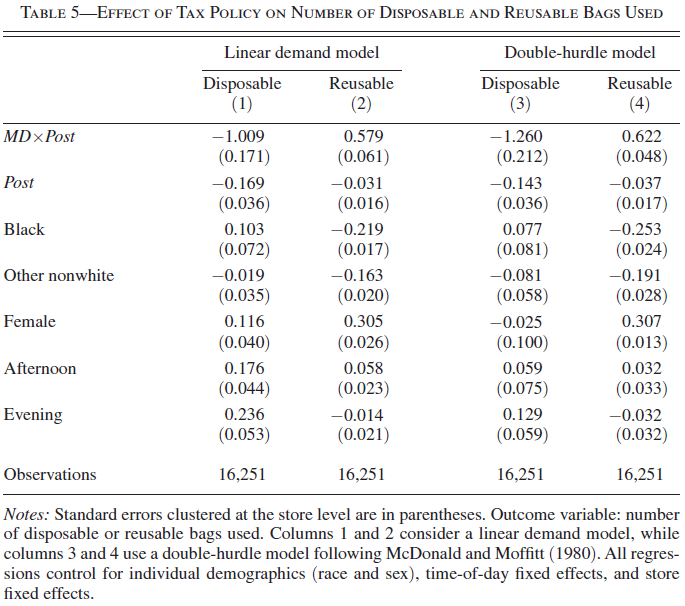
\includegraphics[scale = .8]{0807tanji/T5}
        \end{figure}
      \end{itemize}
      \item The composition of customers shopping may have changed after the implementation: rejected by the scanner data.
    \end{itemize}

    \subsection{Bonus Policy}

    \begin{itemize}
      \item Each sample stores falls into one of four policy types
      \begin{enumerate}
        \item No incentives
        \item offers a bonus but not charge a tax (\$.05)
        \item does not offers a bonus but does charge a tax (\$.05)
        \item both offers a bonus and charges a tax (\$.10)
      \end{enumerate}
      \item The bonus had been introduced before the sample period, so they use cross-sectional comparison.
    \end{itemize}

    \paragraph{Avarage}

    \begin{itemize}
      \item (Organic stores are omitted due to exclude the effect of store-specific characteristics.)
      \item Customers in the stores with/without bonus are similar.
    \end{itemize}


    \begin{itemize}
      \item (Figure 4) Customers in stores with only a bonus used a disposable bag 40.8\%, while that of there with only bonus was 81.9\%.
      \begin{figure}[ht]
        \centering
        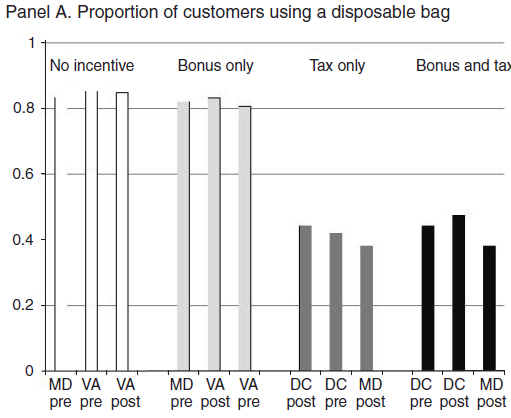
\includegraphics[scale = .8]{0807tanji/F4A}
        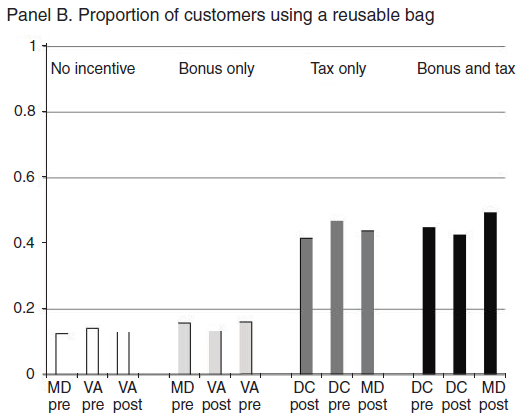
\includegraphics[scale = .8]{0807tanji/F4B}
      \end{figure}
      \item Potential bias: unobserved differences between bonus and non-bonus stores are captured.
      $\Rightarrow$ Suppose that if it were not for bonus, all the consumers shopping at those stores switch to disposable bags: 15.4\%.
    \end{itemize}

    \paragraph{Cross-sectional regression}

    \[
    Y_{isdt} = \alpha + \beta \text{Tax}_{st} + \gamma \text{Bonus}_{s} + \eta Z_s + \gamma X_i + \delta Q_d + \epsilon_{isdt}
    \]

    \begin{itemize}
      \item The magnitude of two incentives differs dramatically.
      \begin{figure}[ht]
        \centering
        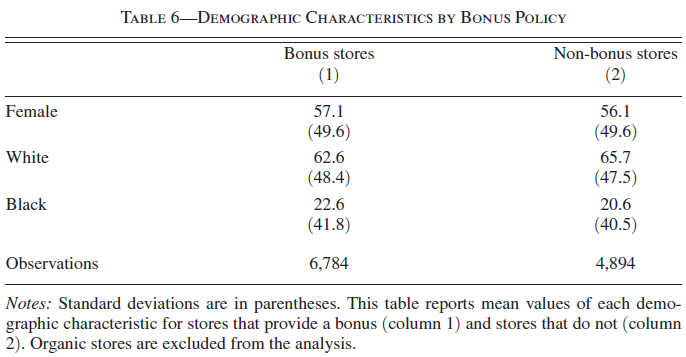
\includegraphics[scale = .8]{0807tanji/T6}
      \end{figure}
      \begin{figure}[ht]
        \centering
        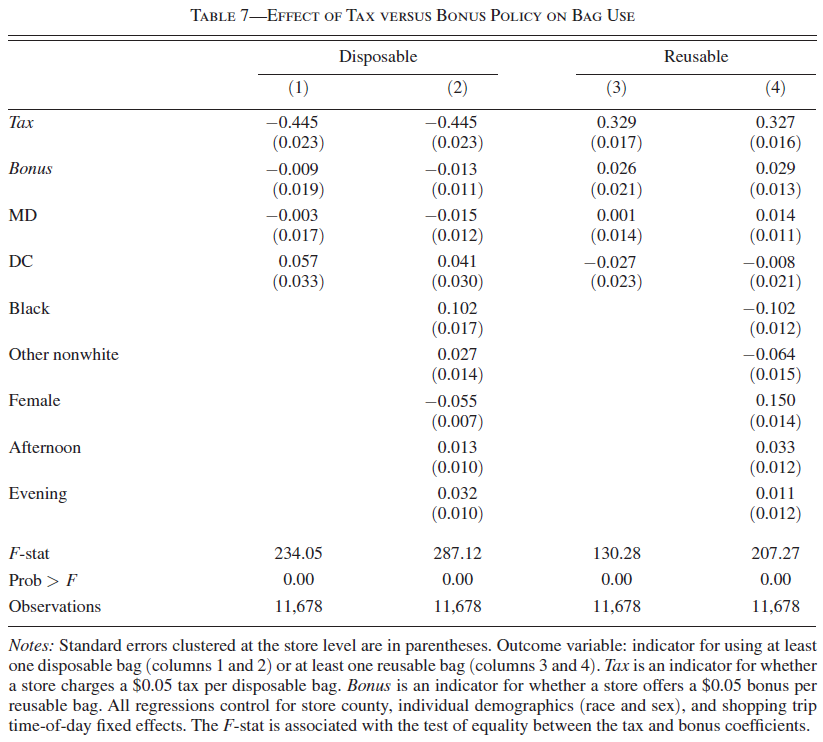
\includegraphics[scale = .8]{0807tanji/T7}
      \end{figure}
    \end{itemize}

    \section{Reasons for Asymmetric Responses to Taxes and Bonuses}

    \subsection{Loss Aversion}

    \begin{itemize}
      \item Recent evidence from the field supports loss-aversion in a wide variety of contexts.
      \begin{itemize}
        \item Labor supply: Camerer et al. 1997; Oettinger 1999
        \item Tax compliance: Rees-Jones 2018; Engstr\"{o}m et al. 2015
        \item Sports performance: Allen et al; Pope and Schweizer 2011
        \item Trading: Odean 1998; Genesove and Mayer 2001.
      \end{itemize}
      \item Studies that use Gain-loss framing as a policy tool to nudge people.
      \begin{itemize}
        \item Fryer et al. (2012) pay-for-performance bonuses for public school teachers.
        \item Hossain and List (2012): productivity bonused for factory workers
        \item Field (2009): tuition subsidies for law students.
      \end{itemize}
      \item Studies above use loss aversion in a more prescriptive way: incentives of quite large amount.
      \begin{itemize}
        \item Several studies show that providing small financial incentives for pro-social behavior actually decrease the desired behavior (Gneezy and Rustichini 2000a, b; Gneezy Meier, and Ray-Biel 2011)
      \end{itemize}
      \item In this paper, customers are loss averse even when the incentives are very small, and no crouding out. (cf. Levitt et al. 2016)
    \end{itemize}

    \subsection{Marketing and Awareness}

    \begin{itemize}
      \item The awareness of the two policies may differ.
      \begin{itemize}
        \item The tax was covered widely in the press in the weeks.
      \end{itemize}
      \item Customers survey revealed:
      \begin{itemize}
        \item Almost all customers were aware of the tax, only half of them in stores with bonus acquainted with the program.
      \end{itemize}
      \item They adjusted this possible bias by rescaling the estimate: devide the estimate by the fraction of customers who were aware of the policy.
      \begin{itemize}
        \item The effect of tax is still than that of bonus: 33.4 vs 5.6 percentage points for the proportion of the customers who use reusable bags.
        \item No more than 9\% of customers who would have switched from disposable to reusable if they had known about the bonus.
      \end{itemize}
    \end{itemize}

    \subsection{Social Norms}

    \begin{itemize}
      \item Two policies may have lead to differential shifts in social norms.
      \begin{itemize}
        \item Tax policy was legislated, while bonus was voluntary.
      \end{itemize}
      \item Survey measures: DID to see the effect of the implementation on the self-reported social norms.
      \begin{itemize}
        \item None of the measures show a significant cgange after the tax was implemented.
      \end{itemize}
      \item Residents of Montgomery County may have been not fully aware of the approval of the law. In addition, they had already experienced the same kind of tax before.
      \begin{figure}[ht]
        \centering
        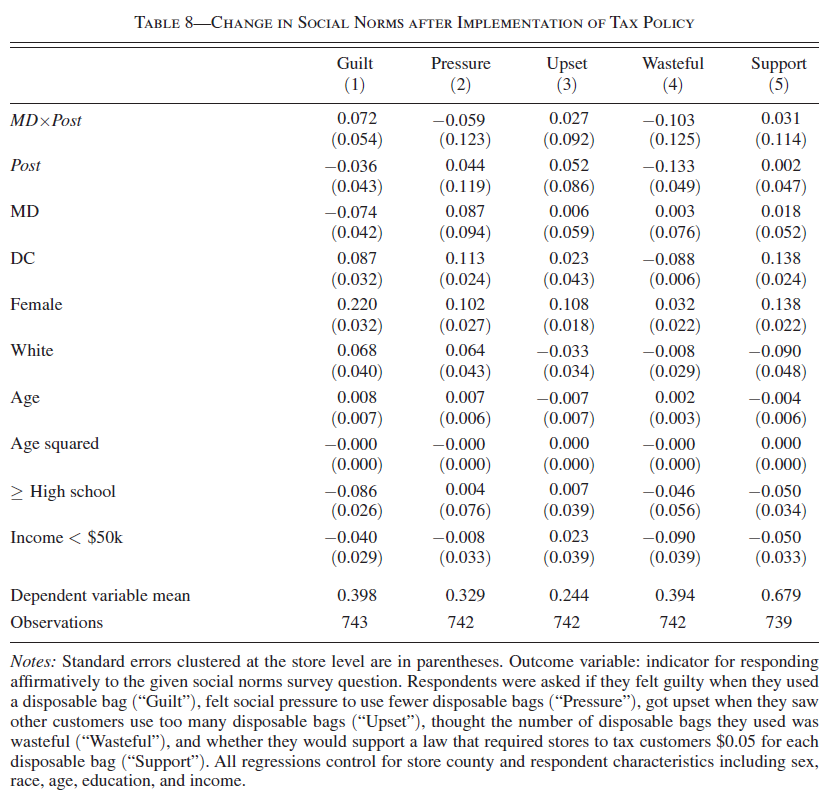
\includegraphics[scale = .8]{0807tanji/T8}
      \end{figure}
    \end{itemize}

    \subsection{Utility from Free Goods}

    \begin{itemize}
      \item An alternative model of reference-dependence
      \begin{itemize}
        \item Individuals get benefits derived from receiving a free product.
        \item As a result, a discontinuous jump occurs in utility at the reference point.
        \[
        u(w_i) = \begin{cases}
          \gamma w_i & \text{ if } w_i \geq w^* \\
          \gamma w_i - \delta & \text{ if } w_{i} < w^*
      \end{cases}, \text{ where } \delta > 0.
        \]
      \end{itemize}
    \end{itemize}

    \subsection{Additional Explanations}

    \begin{itemize}
      \item Asymmetry effect on those who switch to no bags.
      \item The size of reusable bags.
      \item Cashiers may have changed after the implementation: reminder of the tax policy.
      \item "Tax-averion" of the customers.
    \end{itemize}

    \section{Estimating Loss Aversion}

    \subsection{The Coefficient of Loss Aversion}

    \begin{figure}[ht]
      \centering
      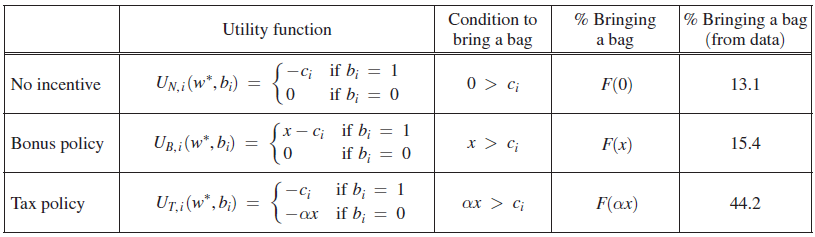
\includegraphics[scale = 1]{0807tanji/model_esti}
    \end{figure}

    \begin{itemize}
      \item We can derive the "coefficient of loss aversion" (Tversky and Kahneman 1991)
      \begin{itemize}
        \item The intrinsic cost of bringing reusable bags are distributed with a normal distribution function $F$, with $\mu = \$.56$ and $\sigma = \$.50$.
        \item This approach yields $\alpha = 5.3$ ($[3.3, 14.8]$ from bootstrapping): To have the same behavioral effect as \$.05 tax by bonus, we have to reward about  \$.25.
      \end{itemize}
    \end{itemize}

    \subsection{Expectations-Based Referenece Points}

    \begin{itemize}
      \item Analyses have been assumed that the customers' reference point of the price of the disposable bags at free.
      \item K\"{o}szegi and Rabin (2006): Reference points are generated by an individual's expectations.
      \item Transaction-level data revealed:
      \begin{itemize}
        \item there are no rebound effect in usage of the disposable bags which may occur when the expectation had been changed in a long run.
      \end{itemize}
      \begin{figure}[ht]
        \centering
        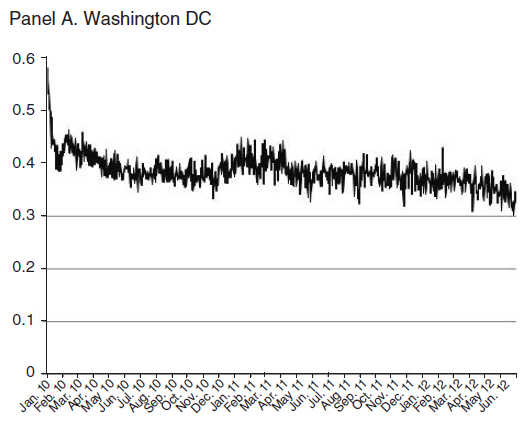
\includegraphics[scale = .8]{0807tanji/F5A}
        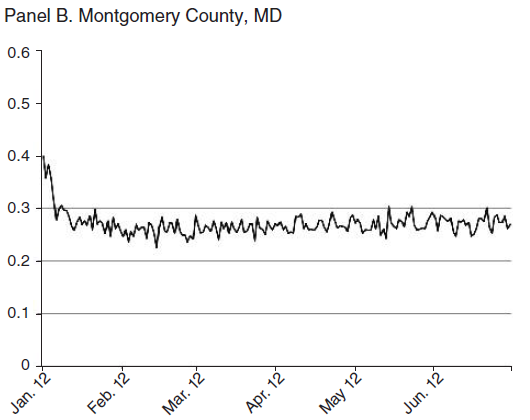
\includegraphics[scale = .8]{0807tanji/F5B}
      \end{figure}
    \end{itemize}


    \section{Conclusion}

    \begin{itemize}
      \item What is interesting is that the effect of this tax is not large.
      \begin{enumerate}
        \item The elasticity of demand for disposable bags is substantially great.
        \item Prominency of the price at grocery store.
        \item Levying a price on a good that had previously been free.
        \item Reputation costs.
      \end{enumerate}
      \item Implications for policy-design.
      \begin{itemize}
        \item discounts to coffee drinkers who use their own bag.
        \item Additional tax credits to customers who purchase Energy Star products.
      \end{itemize}
      \item "a discount and a surcharge are the same thing economically. But we live in a world in which not everyone is an economist" (Liptak 2017)
    \end{itemize}


    %\begin{figure}[]
    %    \centering
    %    \includegraphics{0807tanji/ignore file.txt}
    %    \caption{}
    %    \label{}
    %\end{figure}

    \biblio

\end{document}
